\documentclass[a4paper]{scrartcl}

\usepackage{amsmath, amsthm}
\theoremstyle{definition}
\newtheorem*{example}{Example}
\newtheorem{task}{Task}

\usepackage{url}

\usepackage{tikz}
\usetikzlibrary{arrows}
\tikzset{vertex/.style = {shape=circle,draw,minimum size=1.5em}}
\tikzset{edge/.style = {->,> = latex'}}

\usepackage{nicematrix}
\NiceMatrixOptions{
	code-for-first-row = \color{blue} ,
	code-for-first-col = \color{blue} ,
}

\newcommand*{\mat}[1]{\mathbf{#1}}
\renewcommand*{\vec}[1]{\mathbf{#1}}

\title{MATH280\\ Case 1: PageRank}
\date{}

\begin{document}
	\maketitle
	
	If you haven't done so already, read section 10.1 and 10.2 in \emph{Linear Algebra and Its Applications} (available on Canvas).
	
	\textbf{Note}: In this note, indices start at 0, to correspond with NumPy arrays. If you are using Matlab, vectors and matrices there are 1-indexed, and you have to adjust accordingly.
	
	\section{Directed graphs}
	A directed graph is a set of vertices with directed edges between the vertices.
	\begin{example}[A directed graph]
	\phantom{x}\\
	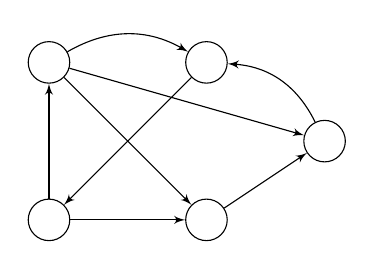
\begin{tikzpicture}
		% vertices
		\node[vertex] (a) at  (0,2) {};
		\node[vertex] (b) at  (2,2) {};
		\node[vertex] (c) at  (3.5,1) {};
		\node[vertex] (d) at  (2,0) {};
		\node[vertex] (e) at (0,0) {};

		%edges
		\draw[edge] (a) to[bend left] (b);
		\draw[edge] (a) to (c);
		\draw[edge] (a) to (d);
		\draw[edge] (b) to (e);
		\draw[edge] (c) to[bend right] (b);
		\draw[edge] (d) to (c);		
		\draw[edge] (e) to (a);
		\draw[edge] (e) to (d);
	\end{tikzpicture}
	\end{example}
	In the PageRank algorithm, each vertex represents a web page, and each edge a link between webpages.
	
	A directed graph can be represented on a computer in several ways. For our purposes, we will focus on the \emph{adjacency matrix}. To form the adjacency matrix of a graph, we first label the vertices of the directed graph with indices  $\{0,1,\dotsc, n-1\}$, where $n$ is the number of vertices.
	
	The adjacency matrix is an $n\times n$-matrix $\mat{A}$, with entries
	\[a_{ij}= \begin{cases} 1 & \text{if there is an edge $i\to j$,}\\
							0 & \text{if not.}
								\end{cases}
	\]
	
	\begin{example}[Adjacency matrix]
		We label the vertices in the graph
		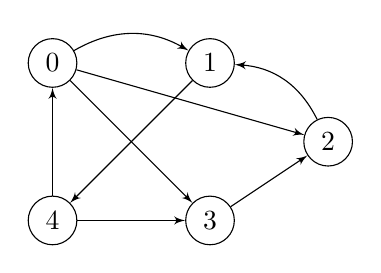
\begin{tikzpicture}

			% vertices
			\node[vertex] (a) at  (0,2) {0};
			\node[vertex] (b) at  (2,2) {1};
			\node[vertex] (c) at  (3.5,1) {2};
			\node[vertex] (d) at  (2,0) {3};
			\node[vertex] (e) at (0,0) {4};
			
			%edges
			\draw[edge] (a) to[bend left] (b);
			\draw[edge] (a) to (c);
			\draw[edge] (a) to (d);
			\draw[edge] (b) to (e);
			\draw[edge] (c) to[bend right] (b);
			\draw[edge] (d) to (c);		
			\draw[edge] (e) to (a);
			\draw[edge] (e) to (d);
		\end{tikzpicture}\\
	To set up the adjacency matrix, we put a 1 at position $(i,j)$ if there is an edge $i\to j$, otherwise we put zero.
	\[
	\mat{A} =\quad   
	\begin{pNiceMatrix}[first-row, first-col]
		   & 0 & 1 & 2 & 3 & 4\\
		 0 & 0 & 1 & 1 & 1 & 0\\
		 1 & 0 & 0 & 0 & 0 & 1\\
		 2 & 0 & 1 & 0 & 0 & 0\\
		 3 & 0 & 0 & 1 & 0 & 0\\
		 4 & 1 & 0 & 0 & 1 & 0
		\end{pNiceMatrix}.
	\]
\end{example}


\section{Transition matrix}
The PageRank Algorithm uses a transition matrix $\mat{P}$ for the random walk across the graph. (See Chapter 10.2 i Lay). This matrix is a stochastic matrix where $p_{ij}$ is the probability of going from state $j$ to state $i$.  


\[
p_{ij}=\begin{cases} \frac{1}{m_j} & \text{if there is an edge $j\to i$}\\
		              0 & \text{otherwise}
	    \end{cases},
\]
where $m_j$ is the number of edges pointing out of node $j$.

\textbf{Note:} The adjacency matrix has $a_{ij}\neq 0$ if there is an edge $i\to j$, while the transition matrix has $p_{ij}\neq 0$ if there is an edge $j\to i$.

To compute $\mat{P}$ from $\mat{A}$ we need to do three things: 
\begin{enumerate}
	\item Compute the number of edges going out from each node.\\
		$m_i=\sum_{j=0}^{n-1}a_{ij}$. 
	\item Divide each row of $\mat{A}$ by the corresponding number of edges, resulting in a matrix $\mat{C}$.\\
		$c_{ij}=\frac{a_{ij}}{m_i}$.
	\item Transpose the resulting matrix.\\
	 	$\mat{P}=\mat{C}^\top$.
\end{enumerate}

\begin{example}[Transition matrix]
	For our example graph, the numbers of edges pointing out of each node are, respectively
	\[
	\vec{m}= 
	\begin{pNiceMatrix}[first-row]
		0 & 1 & 2 & 3 & 4\\
		3 & 1 & 1 & 1 & 2
	\end{pNiceMatrix}
	\]
\end{example}
After dividing each row of $\mat{A}$ and transposing, we end up with the transition matrix $\mat{P}$.

\[
\mat{P}
=\begin{pNiceMatrix}[first-row, first-col]
	& 0 & 1 & 2 & 3 & 4\\
	0 & 0            & 0 & 0 & 0 & \frac{1}{2}\\
	1 & \frac{1}{3}	& 0 & 1 & 0 & 0 \\
    2 & \frac{1}{3}	& 0 & 0 & 1 & 0 \\
	3 & \frac{1}{3} & 0 & 0 & 0 & \frac{1}{2}\\
	4 & 0 			 & 1 & 0 & 0 & 0
\end{pNiceMatrix}.
\]

\begin{task}
	Write a function that takes an adjacency matrix $\mat{A}$ as input, and returns the corresponding transition matrix $\mat{P}$.
\end{task}

\section{The power method}
The PageRank of each node is calculated from the steady-state vector $\vec{q}$, defined by
\[\mat{P}\vec{q} =\vec{q}, \quad\text{and}\quad \sum_{i=0}^{n-1} q_i=1.
\]
As shown in the lectures, 
\[\vec{q}=\lim_{k\to \infty} \vec{x}_k,\]
where $\vec{x}_k$ is a sequence of probability vectors defined by
\[
\vec{x}_{k+1}=\mat{P}\vec{x}.
\]

The idea of the power method is to compute the sequence $\vec{x}_0, \vec{x}_1=\mat{P}\vec{x}_0, \vec{x}_2 =\mat{P}\vec{x}_1, \dotsc$, and use the approximation
\[\vec{q}\approx \vec{x}_N,
\]
for some large $N$.

\textbf{Note:} Here we have assumed that the initial vector $\vec{x}_0$ is a probability vector. If it is not, the sequence will converge to some scalar multiple of $\vec{q}$ instead. 

\begin{task}
	Implement the power method. Your function should take as arguments the transition matrix $\mat{P}$, an initial probability vector $\vec{x}_0$, and the number of iterations $N$.
\end{task}

\begin{example}
For our example graph, $\vec{q}$ can be found by solving the homogenous linear equation $\left(\mat{P}-\mat{I}\right)\vec{q}=0$ and choosing the free parameter such that $\sum_{i=0}^{n-1}q_i=1$.
\[
\vec{q} = \left[\frac{1}{8}, \frac{1}{4}, \frac{5}{24}, \frac{1}{6}, \frac{1}{4}\right]^T.
\]
You can use this to test your method.
\end{example}

\begin{task}
In this task, you are going to test your implementation on a set of webpages and links. This set consists of webpages with an url starting with www.nmbu.no/fakultet/realtek and internal links between them (In January 2022). Dangling nodes have been removed.

The adjacency matrix is stored in `adjacency\_realtek.txt`, and the urls represented by each index in `keyvals.txt`.

What are the top 5 webpages by PageRank on the RealTek webpages?
\end{task}

\section{Additional challenges}

In the power method implemented above, we specify the number of iterations. It would be better to iterate until 
$$\|\vec{x}_{k}-\vec{x}_{k-1}\|\le Tol$$
for some specified tolerance $Tol$.
\begin{task}[a] Implement a new function that does this.
\end{task}
For more efficient code, you should not compute the matrix-vector product $\mat{P}\vec{x}_{k-1}$ more than once per iteration.
It is good practice to implement a maximum number of iterations, so your code doesn't get stuck in an infinite loop.


\setcounter{task}{3}
The actual PageRank algorithm is more robust than what we have done here. By making some adjustments, it can handle dangling nodes (webpages without links) and other complications that may arise.
\begin{task}[b]Implement Adjustment 1 and 2 described in \emph{Linear Algebra and its Applications} Chapter 10.2.
\end{task}

\section{Some additional remarks}
Our implementation only works for graphs with less than a few thousand nodes. For larger graphs, better implementations are needed. Adjacency matrices are usually sparse, that is, most of the entries are zero. Efficient matrix algorithms take advantage of this. In Python, the most used implementation of sparse matrices is scipy.sparse. See \url{https://docs.scipy.org/doc/scipy/reference/sparse.html.}

Really efficient implementations of the PageRank algorithm never explicitly store the adjacency matrix or the transition matrix. It is possible to compute a matrix-vector product $\mathbf{P}\mathbf{v}$ using only the adjacency list (\url{https://en.wikipedia.org/wiki/Adjacency_list}) of the graph.

\end{document}